\documentclass[a4paper,UKenglish]{lipics-v2016}
%This is a template for producing LIPIcs articles. 
%See lipics-manual.pdf for further information.
%for A4 paper format use option "a4paper", for US-letter use option "letterpaper"
%for british hyphenation rules use option "UKenglish", for american hyphenation rules use option "USenglish"
% for section-numbered lemmas etc., use "numberwithinsect"
 
\usepackage{microtype}%if unwanted, comment out or use option "draft"

%\graphicspath{{./graphics/}}%helpful if your graphic files are in another directory

%My packages
%\usepackage{amsthm}

%\theoremstyle{definition}
%\newtheorem{definition}{Definition}[section]


\bibliographystyle{plainurl}% the recommended bibstyle

% Author macros::begin %%%%%%%%%%%%%%%%%%%%%%%%%%%%%%%%%%%%%%%%%%%%%%%%
%\title{Robust Estimation and Comparison of Origin-Destination Flows with Data Depth}\footnote{A full version of the paper is available at \cite{DBLP:journals/cacm/Knuth74}, \url{XXX}}}
\title{Outliers Detection and Comparison of Origin-Destination Flows with Data Depth}
\titlerunning{Outliers Detection and Comparison of Origin-Destination Flows with Data Depth} %optional, in case that the title is too long; the running title should fit into the top page column

%% Please provide for each author the \author and \affil macro, even when authors have the same affiliation, i.e. for each author there needs to be the  \author and \affil macros
\author[1]{Myeong-Hun Jeong}
\author[2]{Junjun Yin}
\author[3]{Shaowen Wang}
\affil[1]{Department of Civil Engineering,  Gwangju, Republic of Korea\\
  \texttt{mhjeong@chosun.ac.kr}}
\affil[2]{Social Science Research Institute, Penn State University, PA, USA\\
  \texttt{jyin@psu.edu}}
\affil[3]{Departmet of Geography and Geographic Information Science, the University of Illinois at Urbana-Champaign, IL, USA\\
	\texttt{shaowen@illinois.edu}}
\authorrunning{M.-H. Jeong, J. Yin and S. Wang} %mandatory. First: Use abbreviated first/middle names. Second (only in severe cases): Use first author plus 'et. al.'

\Copyright{Myeong-Hun Jeong, Junjun Yin, and Shaowen Wang}%mandatory, please use full first names. LIPIcs license is "CC-BY";  http://creativecommons.org/licenses/by/3.0/

\subjclass{Dummy classification -- please refer to \url{http://www.acm.org/about/class/ccs98-html}}% mandatory: Please choose ACM 1998 classifications from http://www.acm.org/about/class/ccs98-html . E.g., cite as "F.1.1 Models of Computation". 
\keywords{Dummy keyword -- please provide 1--5 keywords}% mandatory: Please provide 1-5 keywords
% Author macros::end %%%%%%%%%%%%%%%%%%%%%%%%%%%%%%%%%%%%%%%%%%%%%%%%%

%Editor-only macros:: begin (do not touch as author)%%%%%%%%%%%%%%%%%%%%%%%%%%%%%%%%%%
\EventEditors{John Q. Open and Joan R. Acces}
\EventNoEds{2}
\EventLongTitle{42nd Conference on Very Important Topics (CVIT 2016)}
\EventShortTitle{CVIT 2016}
\EventAcronym{CVIT}
\EventYear{2016}
\EventDate{December 24--27, 2016}
\EventLocation{Little Whinging, United Kingdom}
\EventLogo{}
\SeriesVolume{42}
\ArticleNo{23}
% Editor-only macros::end %%%%%%%%%%%%%%%%%%%%%%%%%%%%%%%%%%%%%%%%%%%%%%%

\begin{document}

\maketitle

\begin{abstract}
Abstract

 \end{abstract}

\section{Introduction}

With the rapid rise in ubiquity of geo-tagged sensors, knowledge discovery power is enhanced by extracting interesting patterns from spatiotemporal big data in various domains. In particular, the location-acquisition technologies generate large volumes of movement data such as people, animals, vehicles and natural phenomena. These big movement data help us understand moving objects, and discover the hidden patterns. Thus, trajectory mining leads to solutions for important research problems in different fields such as urban planning \cite{mazimpaka15AGILE}, transportation \cite{chen13Percom}, environment \cite{devarakonda13SIGKDD}, and public security and safety \cite{buchin14JOSIS}.

This paper presents a new algorithm which not only estimates origination-destination (OD)'s flows anomaly but also conducts hypothesis testing between two different OD flows. This paper utilizes a New York City Taxi data set that has the origin and destination of each movement without the whole actual trajectory routes. The analysis of digital footprints obtained from taxi data has a crucial role in  understanding crowd patterns and planning urban and transportation investments in administrative authorities.


In recent years, researchers have investigated a variety of approaches to trajectory data mining. There are generally four categories that classify trajectory mining methods: clustering, classification, frequent/group pattern mining, and outlier detection \cite{mazimpaka16JOSIS,zheng15ACMTIST}. These techniques can be used independently or combinatorially for trajectory mining application problems. 

In particular, this study focuses on outlier detection of OD flows. Outlier detection aims to find trajectories that do not follow the typical flow of trajectory data sets for characterizing the connectivity between regions \cite{mazimpaka16JOSIS}. \cite{fontes13GeoInfo,lee08ICDE} use Euclidean distance to find outlier patterns from trajectories.  \cite{pan13ACMGIS,liu12IJGIS} raise the questions of Euclidean distance approach due to the loss of local features and unavailability when external factors affect the trajectories (e.g., topography, land cover or weather condition).  \cite{pan13ACMGIS,liu12IJGIS} addresses this by using robust distance measurements (i.e., Mahalanobis distance \cite{pan13ACMGIS} and relative distance  \cite{liu12IJGIS}). Further, structural features  \cite{yuan11JCIS} and a data-induced random tree  \cite{zhang11UC} are exploited to detect anomalous trajectories instead of using distance or density. In a similar fashion, this study considers the center regions of OD flows with data depth in order to robustly detect the trajectory outliers. 



In addition, visual analytics are a common approach to analyze OD flow data. Visual representation of massive movement data enables comprehensive exploration of data and results in understanding complex flow trends. Aggregation and generalization of movement data are frequently utilized \cite{andrienko08VAST,adrienko11IEEETVCG,guo14IEEETVCG}. While visual analytics can help to extract inherent patterns from massive data, it is difficult to compare two different OD flows based on a hypothesis testing. In other words, it is complicated to comprehend how two OD flows differ and by how much. This paper uses bivariate hypothesis testing methods based on data depth to understand how different two OD flow data sets are in terms of the amount of spatial extent and a shift in location. 


Further, flow mapping approaches frequently suffer from the modifiable area unit problem (MAUP). For instance, it is not guaranteed that different aggregations via location can present coherent patterns. Kernel-based flow estimation and smoothing are used to overcome different spatial resolution \cite{guo14IEEETVCG}. This study uses traffic analysis zones in New York City as a base unit. Thus, it does not consider MAUP problem. In addition, New York City Taxi data includes the origin and destination within traffic analysis zones, which ignores the actual trajectory route. It is not necessary to reconstruct individual movements for flow estimation (see \cite{duckham16ICGIS}).

In summary, this paper presents a new algorithm which conducts outlier detection as well as a hypothesis testing from OD flows data. Our approach investigates the central regions of  OD flows based on data depth to detect OD flows anomaly and conduct a hypothesis testing between two different OD flow data sets. 

In the remainder of this paper, Section \ref{sec:methods} overviews how to detect OD flows outliers and conduct  a hypothesis testing between two different OD flows with the concept of data depth. Experimental design and the evaluation of the algorithm are presented in Section \ref{sec:experiments}. These results are discussed in Section \ref{sec:discussion}. Section 5 concludes with a summary and future perspectives.


%However these approaches take into account whole trajectories or sections of trajectories based on applications. This study focuses on OD flow data, which ignores the actual trajectory route. Additionally, it is not necessary to reconstruct individual movements for flow estimation (see \cite{duckham16ICGIS}). Further, this study considers spatial association of OD flow patterns with data depth to detect trajectory outliers. However, this study focuses on OD flow data, which ignores the actual trajectory route. The methods mentioned above consider the whole trajectory route. Further, New York City Taxi data have obivious  
%Clustering techniques are used to analyze the moving objects such as daily travel in a city and cyclone tracks \cite{rinzivillo12KI,gaffney07CD}. Human mobility is represented as a network with clustering technique \cite{liu09CUPUM}.  

%Trajectory pattern mining.//
%clustering//
%Outliers//
%
%
%Trajectory clustering can be applied on either whole trajectories or sections of trajectories
%depending on the goal of analysis and the similarity function applied. For example, if
%the similarity function is defined as similar origin and similar destination, the trajectories
%can be clustered as a whole because the route followed is not important.
%
%
%visualization//
%
%Statistical testing//
%
%MAUP problems, uncertainty//
%
%make no attempt to 
%
%
%The  rapid growth of geospatial data results in enhancing knowledge discovery power by extracting interesting patterns from big data in various domains. There are many mining and analysis methodologies to extract new insights from observed data. In particular, this paper investigates spatio-temporal pattern maps that enable hypothesis testing to understand how groups differ and by how much. 
%
%In addition, our approach provides a method to comparing two independent groups based on data depth. The typical KDE can not provide its statistically significant difference between two different density maps. This study provides how different two data sets are in terms of the amount of scale and a shift in location. These features provide an interesting and useful perspective when trying to characterize how group differ. 
%However, the current study is specifically designed to deal with the entire area between two data sets. It is necessary to expand our approach to investigate local variations. Further, work might also test and compare with alternatives such as a spatial scan. 
%
%Our approach can take into account the overall structure of the data. This method can contribute to gaining a better understanding of data in a variety of applications such as influenza spread map or radiation level changes.
%
%The rapid growth of geospatial data can result in enhancing knowledge discovery power by
%extracting interesting patterns from big data in various domains. The identification of statistically significant hot spots has become a key problem that numerous businesses and organizations are attempting to solve. There are many spatial data mining and analysis methodologies to extract unusual patterns of data. This paper proposes a new spatiotemporal hypothesis testing using data depth. This study investigates how much two independent data sets are different in terms of the amount of spatial extent and a shift in location. These features provide an interesting and useful perspective when trying to characterize how groups differ. The experimental comparison with the leading state-of-the-art alternatives demonstrates that the proposed algorithm can not only take into account the overall structure of the data such as hot spots of drop-off locations in the New York City Taxi data, but also conducts statistical hypothesis testing. This method can contribute to gaining a better understanding of data in a variety of applications.



\section{Methods}
\label{sec:methods}
%We further develop a set of well thought out techniques to improve the performance.

\subsection{Data Depth}
Data depth measures the centrality of a point with regard to a given data sets in $\mathbb{R}^d$.  The notion of data depth (i.e., Tukey's halfspace depth) is originally developed by \cite{tukey75ICM}, which generalizes the univariate concept of ranking to multivariate data. It presents how deeply a point is located within a given data sets by ordering their degree of centrality. 

In general, the halfspace depth (HD) of a point $x$ in  $\mathbb{R}^d$ is defined as the minimum probability, $P$ on  $\mathbb{R}^d$, associated with any closed halfspace containing $x$ \cite{liu00AS}. 
\begin{equation*}\label{eq:hd}
HD(x;P) = inf\{P(H): \text{H a closed halfspace}, x \in H\}\text{, } x \in \mathbb{R}^d.
\end{equation*}

For the univariate case, all values less than or equal (greater than or equal) to $x$ form a closed halfspace. 
In Figure \ref{fig:hd_uni}, the probability of values less than or equal to 4 is  $2/7$ and the probability greater than or equal to 4 is $6/7$. The halfspace depth of 4 is $2/7$ which is the minimum probability carried by any closed halfspace containing 4. Further, 14 has the largest halfspace depth, which is the usual sample median. However, the polluted point inflates the standard error of the sample mean, thereby giving a distorted view of the data. 


\begin{figure}
	\centering
	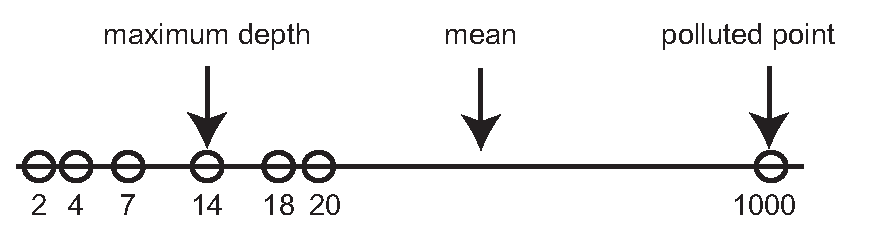
\includegraphics[width=0.8\textwidth]{images/depth_uni.eps}
	\caption{Robustness of halfspace depth for the univariate case}
	\label{fig:hd_uni}	
\end{figure}


In a similar fashion, the halfspace depth of $x$ for the bivariate case is defined as the minimal number of data points in any closed halfspace, determined by a hyperplane through $x$ \cite{rousseeuw96RSS}. For example, the line through $x$ is rotated by $180^{\circ}$ in Figure \ref{fig:hd_bi}. The halfspace depth of $x$ is determined by the smallest portion of data that are separated by such a hyperplane (e.g.,  the halfspace depth of $x$ is $3/13$, determined by the dotted line).
 
\begin{figure}
	\centering
	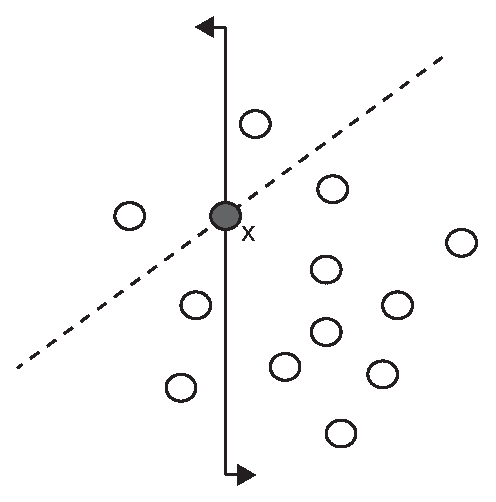
\includegraphics[width=0.6\textwidth]{images/depth_bi.eps}
	\caption{Halfspace depth for the bivariate case}
	\label{fig:hd_bi}	
\end{figure}

The property of halfspace depth is a center-outward ordering of points in  $\mathbb{R}^d$ and affine invariant \cite{Mosler13book}. These features serve as a useful tool in nonparametric inference, which lead to various applications such as data classification and clustering analysis
\cite{lange14fSP,jeong16acmgis}. There are a couple of approaches to calculate data depth: halfspace detpth \cite{rousseeuw96RSS}, projection depth \cite{wilcox03CSSC}, and simplicial depth \cite{liu90AS}. While the computational complexity of the projection approach is $\mathcal{O}(n^2)$ (where $n$ is the number of points), the computational complexity of simplicial depth is $\mathcal{O}(n^3)$. This can significantly increase execution time when $n$ is large. Thus, this paper uses the halfspace depth fuction proposed by \cite{rousseeuw96RSS} of which computation complexity is $\mathcal{O}(n\log{}n)$.



\subsection{OD Trajectory Outlier Detection Based on Depth}
The center-outward ordering in data depth is closely related to the detection of outliers. The upper level sets of data depth in $\mathbb{R}^2$ form the central regions. The most central region can be regarded as a median. Conversely, the lower level sets of data depth, coincide with large distance from the center, can be regarded as outlyingness. \cite{rousseeuw99AS,aplpackR} utilizes this concept to generate a bag plot, which is analogous to the one-dimensional box plot based on data depth. This paper uses the bag plot in order to identify the outliers of OD flows. Before explaining the method of outliers detection, we define a couple of definitions.

%\theoremstyle{definition}
\begin{definition}{Point.}
	A point $p$ is a tuple $(o,d,t)$, where $o$ and $d$  are the origin and destination ID of  traffic analysis zones and $t$ is the time when the destination ID is recorded.
\end{definition}


\begin{definition}{Trajectory.}
	A trajectory $TR$ is a list of points $(p_1, p_2, p_3,...,p_n)$, where $p_i = (o_i,d_i,t_i)$ and $t_1<t_2<t_3<...<t_n$.
\end{definition}

\begin{definition}{OD flow.}
	A OD flow $OD$ is a sum of subset of trajectory $TR$. $OD = (OD_1, OD_2, OD_3,...,OD_k)$, where $OD_i = (o_i,d_i,c_i,ts_i, te_i)$, where $c_i$ is the count of the same origin ID ($o_i$) and destination ID ($d_i$) between the start time ($ts_i$) and the end time ($te_i$), $ts_i<te_i$.
\end{definition}

Based on these basic definitions, we plot the OD flows of New York City Taxi data (May 21 and July 01 2014) using a bag plot in Figure \ref{fig:bagplot_0521_0701}. In Figure \ref{fig:OD_0521}, the deepest depth of OD flows (i.e., depth median) is represented as a star symbol. This point is surrounded by a bag, which contains the half of OD flows (dark blue area). Magnifying the bag by a factor of 3 relative to depth median constructs a fence (light blue area). The fence is comparable with whiskers in an one-dimensional boxplot. The OD flows outside the fence are outliers (red color circles). The x-axis indicates the counts of forward OD flows and the y-axis indicates  the counts of reverse OD flows in Figure \ref{fig:OD_0521}. We can similarly present the bag plot of July 01 2014 in Figure \ref{fig:OD_0721}.


\begin{figure}
	\centering
	\begin{subfigure}[b]{0.49\textwidth}
		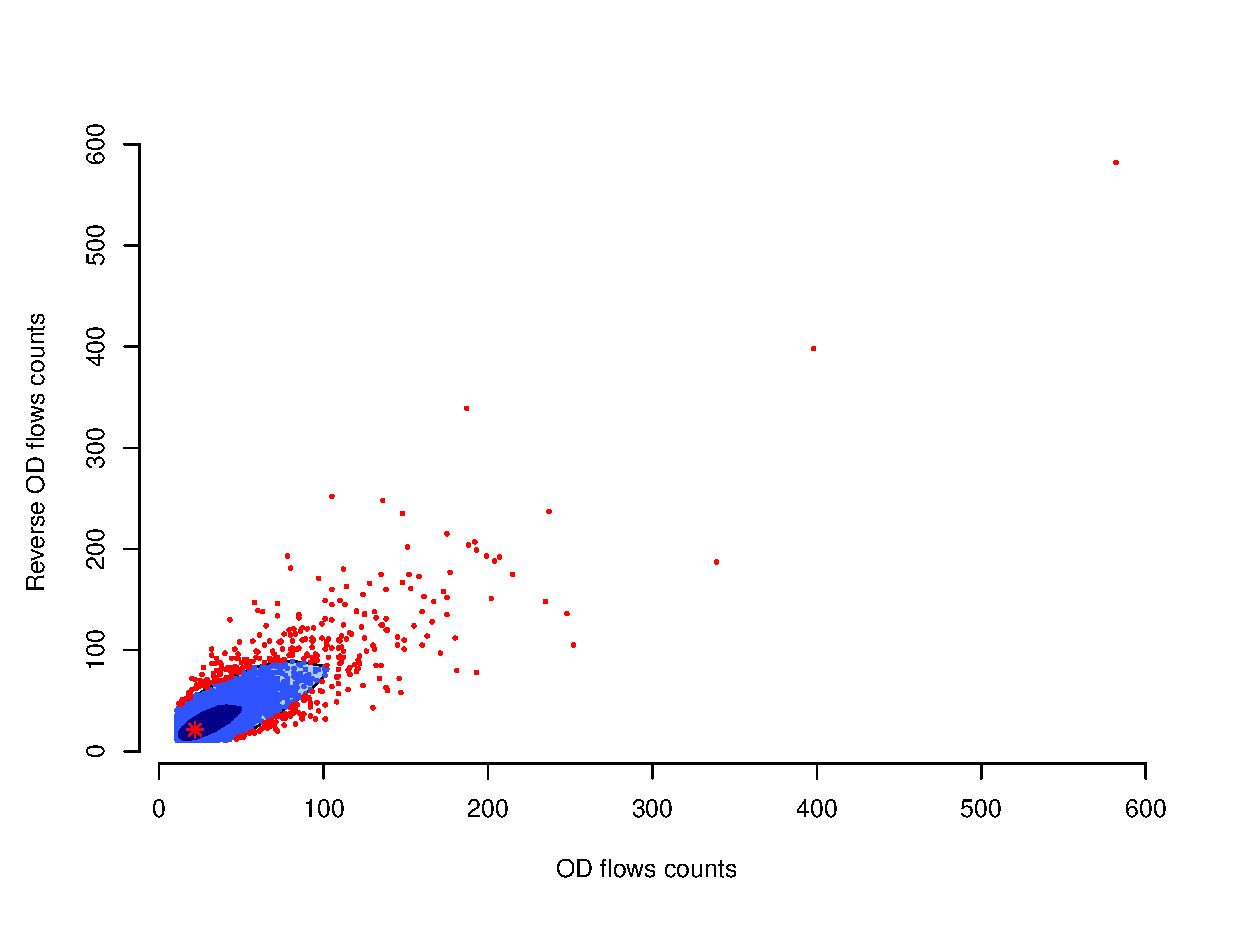
\includegraphics[width=\textwidth]{images/OD_0521.eps}
		\caption{May 21 2014}
		\label{fig:OD_0521}
	\end{subfigure}
	\hfill %add desired spacing between images, e. g. ~, \quad, \qquad, \hfill etc. 	%(or a blank line to force the subfigure onto a new line)
	\begin{subfigure}[b]{0.49\textwidth}
		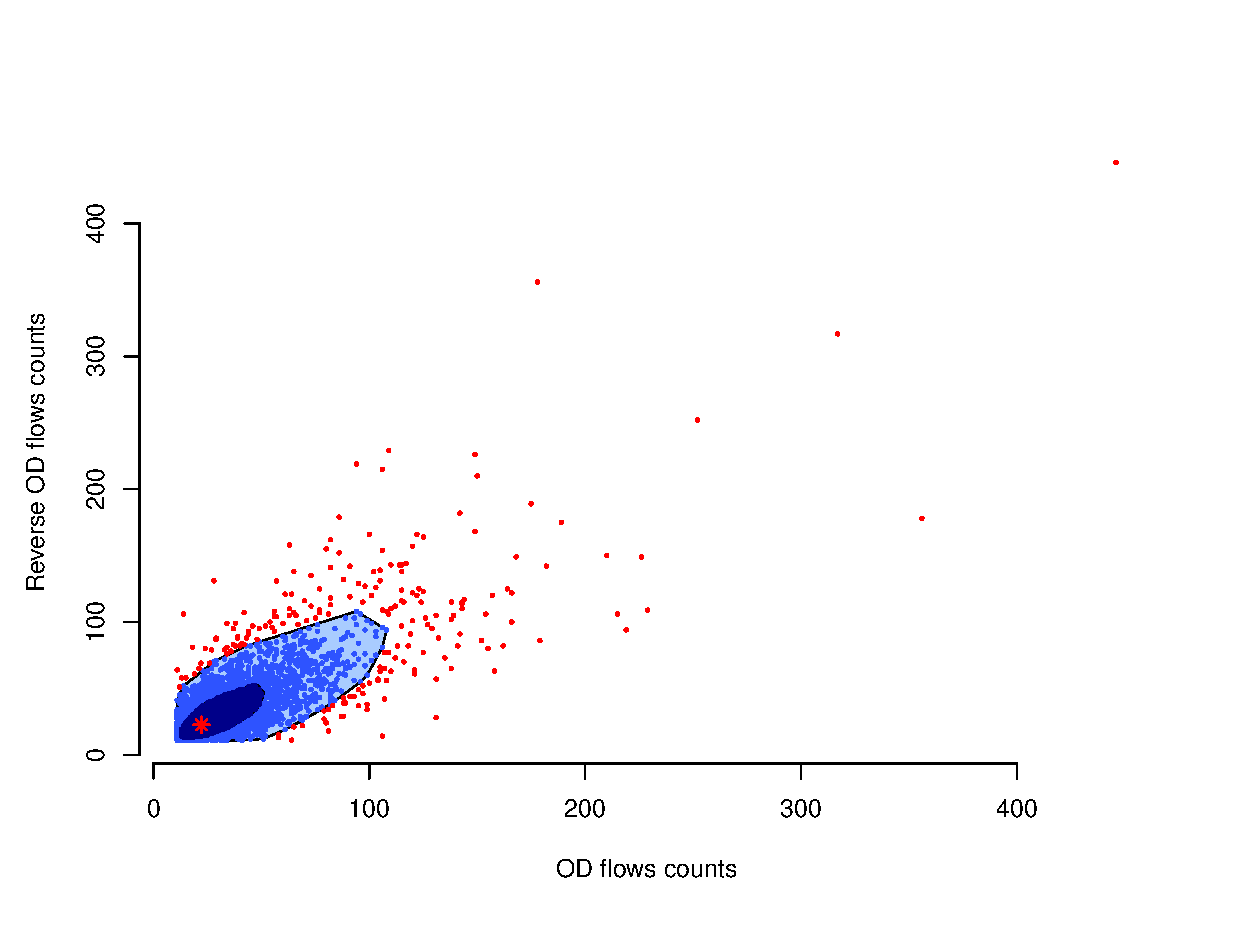
\includegraphics[width=\textwidth]{images/OD_0701.eps}
		\caption{July 01 2014}
		\label{fig:OD_0721}
	\end{subfigure}
    \hfill
	\begin{subfigure}[b]{0.49\textwidth}
	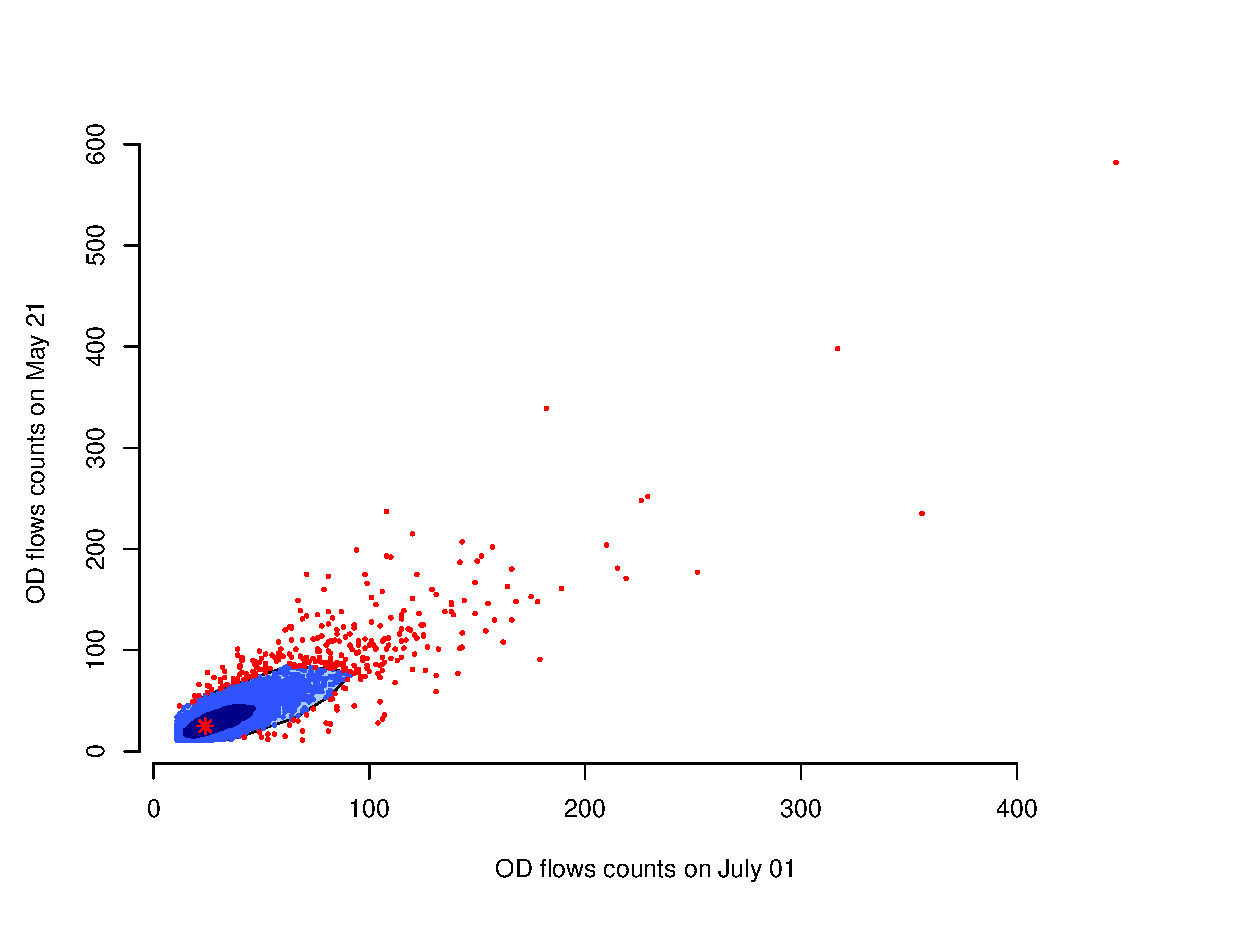
\includegraphics[width=\textwidth]{images/OD_0701_0521.eps}
	\caption{Combination of May 21 and July 01}
	\label{fig:OD_0721_0521}
	\end{subfigure}
    \hfill
	\begin{subfigure}[b]{0.49\textwidth}
	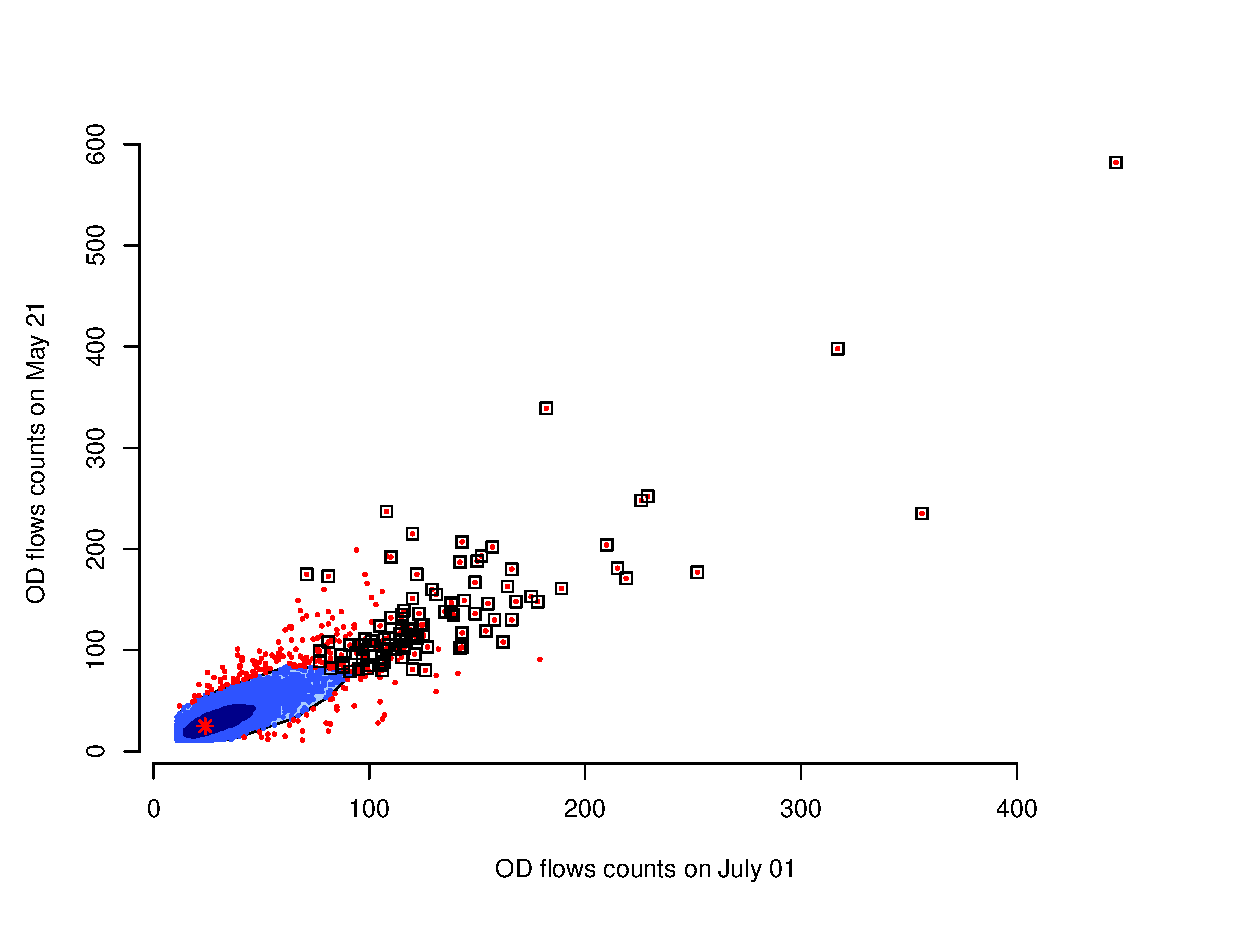
\includegraphics[width=\textwidth]{images/Outliers_high_0701_0521.eps}
	\caption{Detection of outliers for high volume of trips}
	\label{fig:OD_outliers_high}
    \end{subfigure}
	\begin{subfigure}[b]{0.53\textwidth}
	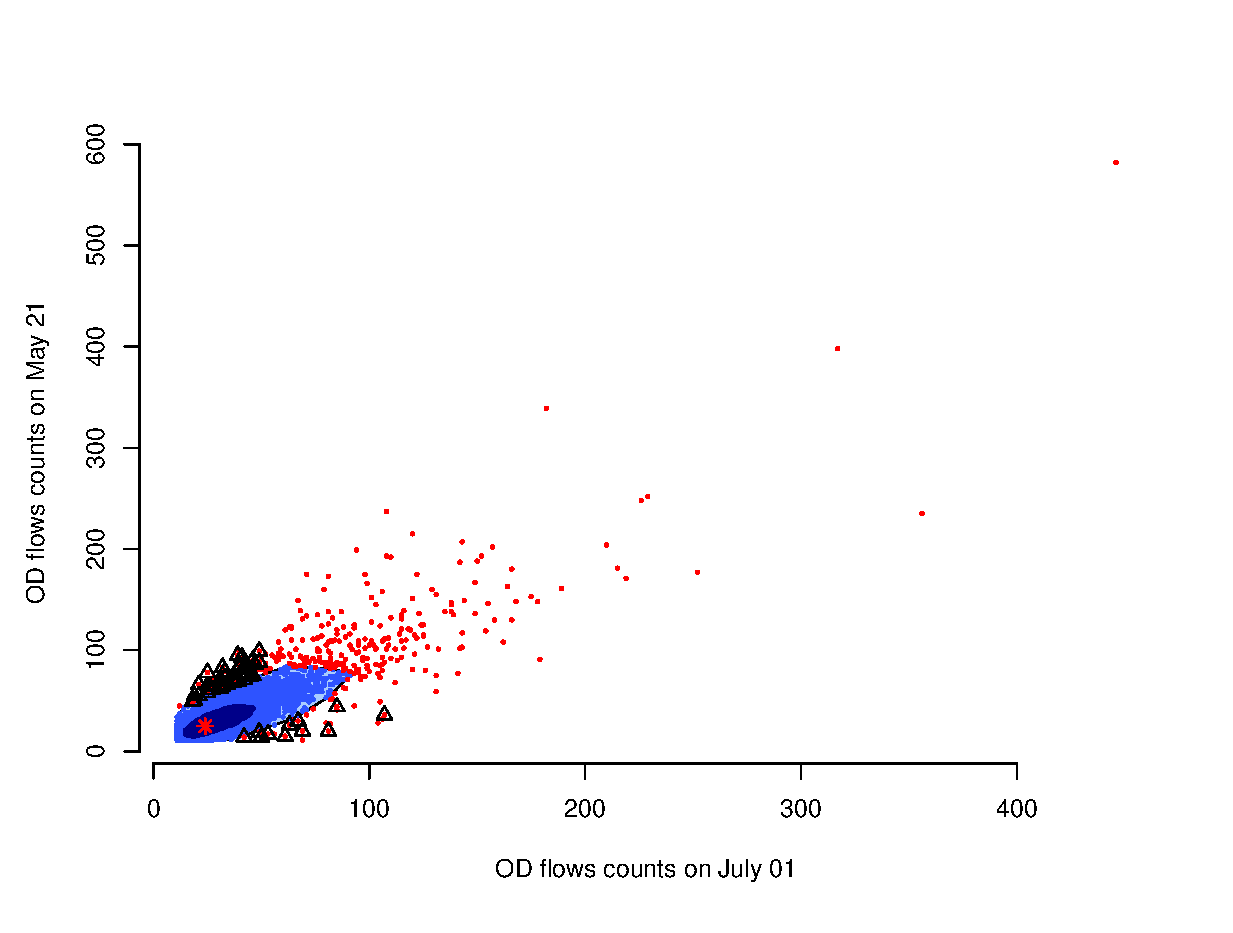
\includegraphics[width=\textwidth]{images/Outliers_rare_0701_0521.eps}
	\caption{Detection of outliers for atypical OD flow patterns}
	\label{fig:OD_outliers_rare}
    \end{subfigure}
	\caption{Outliers detection of OD flows using a bag plot}\label{fig:bagplot_0521_0701}	
\end{figure}

The bag plot is able to present the location (the depth median), spread (the size of bag), correlation (the orientation of the bag), and skewness (the shape of the bag and the fence) of data \cite{rousseeuw99AS}. For example, we can see which forward OD flows have higher counts compared with reverse OD flows; the relatively linear correlation between forward OD flows and reverse OD flows; and the skewness of forward (reverse) OD flows in Figure \ref{fig:OD_0521}. 

In addition, it is possible to detect the outliers of OD flows of two different time stamps. In Figure \ref{fig:OD_0721_0521}, we visualize the OD flows of two different days. Thus, we can not only see where is the central region of OD flows, but also differentiate which OD flows are significantly different compared with two different OD flows.

Further, the OD flows of high active areas in a city are more likely to have large volume of trips. We use set operations to detect such outliers. For example, we regard OD flows on July 01  as control data set ($control$); OD flows on May 21 as test data set ($test$); and the combination of two OD flows as combination data set ($combination$) in Figure \ref{fig:bagplot_0521_0701}. Then we can calculate the intersection of three outliers sets ($control \cap test \cap combination$), which are represented as rectangle symbols in Figure \ref{fig:OD_outliers_high}. 

In addition, it is interesting to detect the outliers of OD flows which are typical patterns at time $t_1$ and atypical behavior at time $t_2$.  For example, we define the union of points in the bag at time $t_1$ and $t_2$. Then we can calculate the intersection of two sets: the outliers of combination set and the previous union set. These outliers are represented as triangle symbols in Figure \ref{fig:OD_outliers_rare}. For example, these outliers are typical OD flows at time $t_1$ which are located in the central regions in the bag plot. When we consider two OD flows together, they become unusual OD flows (e.g., some have more trips and some have less trips compared with the control data set). Thus, we can detect and treat outliers in an interactive way based on data depth.

% we regard OD flows on July 01 ($t_1$) as control data set($control$) and OD flows on May 21 ($t_2$) as test data set ($test$). From the combination of two OD flows set ($combination$, see Figure \ref{fig:OD_0721_0521}), we calculate the interaction of the combination of two OD flows set and the test data set ($B = \{combination \cap test\}$). We also calculate the difference between the combination of two OD flows set and the control data set ($A = \{combination - control\}$) . Finally, we can detect the outliers of OD flows based on the difference between two sets $A$ and  $B$ ($C = \{A - B\}$). The triangles indicate these outliers in Figure \ref{fig:OD_outliers}.

\subsection{OD Trajectory Comparisons Based on Depth}
Data depth can compare bivariate data related with two independent groups \cite{liu93JASA}. A t-test can be used to compare two means from independent groups. For example, the t-test reveals whether two OD flows' means  are different at two different time stamps. However, it is worth examining how groups differ in terms of scale. The comparisons of central regions in data depth compare the marginal distribution, thereby considering the overall structure of the data \cite{wilcox03MBR}.

Let $X$ and $Y$ be the random variables having distributions F and G for two independent groups. The quality index proposed by \cite{liu93JASA} is the probability that the depth of $Y$ is greater than or equal to depth of $X$. 

\begin{equation*}
Q(F,G) = P[D(X;F) \leq D(Y;F)],
\end{equation*}

where $P$ is the probability and $D(X;F)$ is the depth of a randomly sampled observations according with the distribution $F$. \cite{liu93JASA} presents the range of $Q$ is $[0,1]$ and $Q(F,G) = 0.5$ if and only if $F = G$. If $Q < 0.5$  or $Q > 0.5$, a scale increases or decreases from  $F$ to $G$.   It is therefore possible to detect differences in scale based on a bootstrap method.

Let $X_1,...,X_a$ be a random sample from $F$, and $Y_1,...,Y_b$ be a random sample from $G$. The estimate of $Q(F,G)$ is as below.

\begin{equation*}
\hat{Q}(F,G) =\frac{1}{b} \sum_{i=1}^{b} R(Y_i;F_a),
\end{equation*}

where $R(Y_i;F_a)$ indicates the proportion of $X_j$ which has $D(X_j;F_a) \leq D(Y_i;F_a)$. Similarly, the estimate of $Q(G,F)$ can be defined as below.

\begin{equation*}
\hat{Q}(G,F) =\frac{1}{a} \sum_{i=1}^{a} R(X_i;G_b).
\end{equation*}

Bootstrap samples are obtained by resampling from the two groups ($F$ and $G$). Under the null hypothesis ($H_0: Q(F,G) = Q(G,F)$), the difference of the resulting bootstrap estimates is $Q^*(F,G) - Q^*(G,F)$. Thus, if the confidence interval of $Q(F,G) - Q(G,F)$ does not contain zero, we can reject the null hypothesis, $H_0$ \cite{liu93JASA,wilcox03MBR}.

\begin{figure}
	\centering
	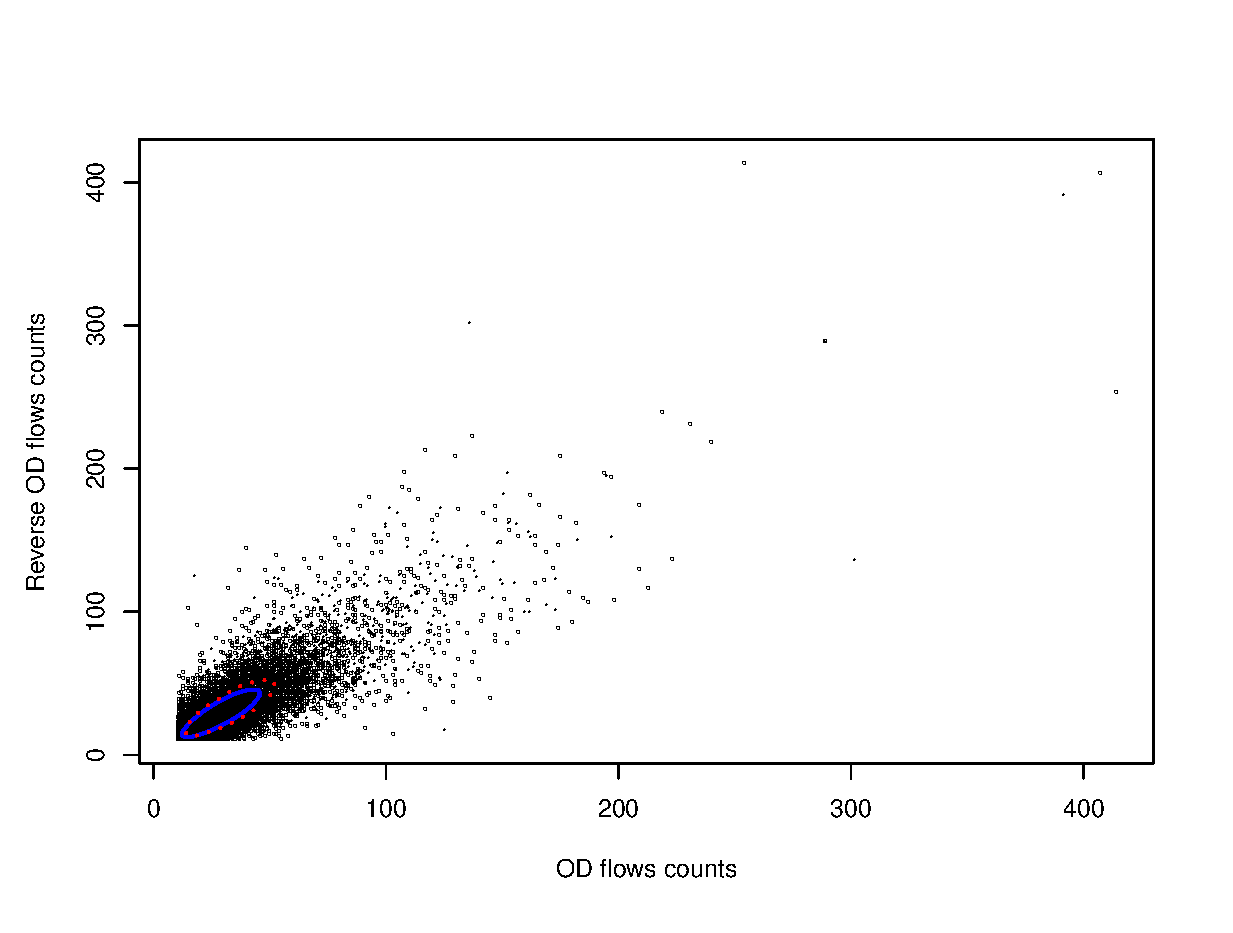
\includegraphics[width=0.6\textwidth]{images/com_mar_0329.eps}
	\caption{Central regions of two OD flows: $\circ$ indicates the OD flows for Saturday, March 29 2014 and * indicates the OD flows for a list of Saturdays; blue line presents the central region of the OD flows for the list of Saturdays and red dotted line presents the central region of the OD flows on March 29.}
	\label{fig:com_mar_0329}	
\end{figure}

For ease of understanding, Figure \ref{fig:com_mar_0329} presents the central regions of two OD flows. One data set is OD flows for Saturday, March 29 2014 and the other is Saturday data sets which include March  1, 8, 15, 22, and April 5. March 29 has the highest number of taxi trips of the year (i.e., 552,064 taxi trips).  The data set for the list of Saturdays has 2,621,703 taxi trips. The bootstrap method reveals that the confidence interval is 0.02467486 and 0.0595938. This confidence interval does not include zero, which results in rejecting the $H_0$. This means that the amount of scale is significantly changed between two OD flows. 

In addition, it is apparent that the bootstrap method is a time consuming process. We generate $2,000$ bootstrap samples. In order to scale up the bootstrap computation, we spread work across multiple nodes and cores by implementing an embarrassingly parallel R code.  Thus, we investigate resource pressures between serial and parallel approaches in the following section.



\section{Experiments}
\label{sec:experiments}

\subsection{Data}
This study uses New York City Taxi data in 2014 to evaluate the effectiveness of the proposed approach.
Figure \ref{fig:taxizone} presents taxi analysis zones in New York City which indicates the origin and the destination IDs of OD flows. Figure \ref{fig:ODflows} shows OD flows on July 01. 

\begin{figure}
	\centering
	\begin{subfigure}[b]{0.49\textwidth}
		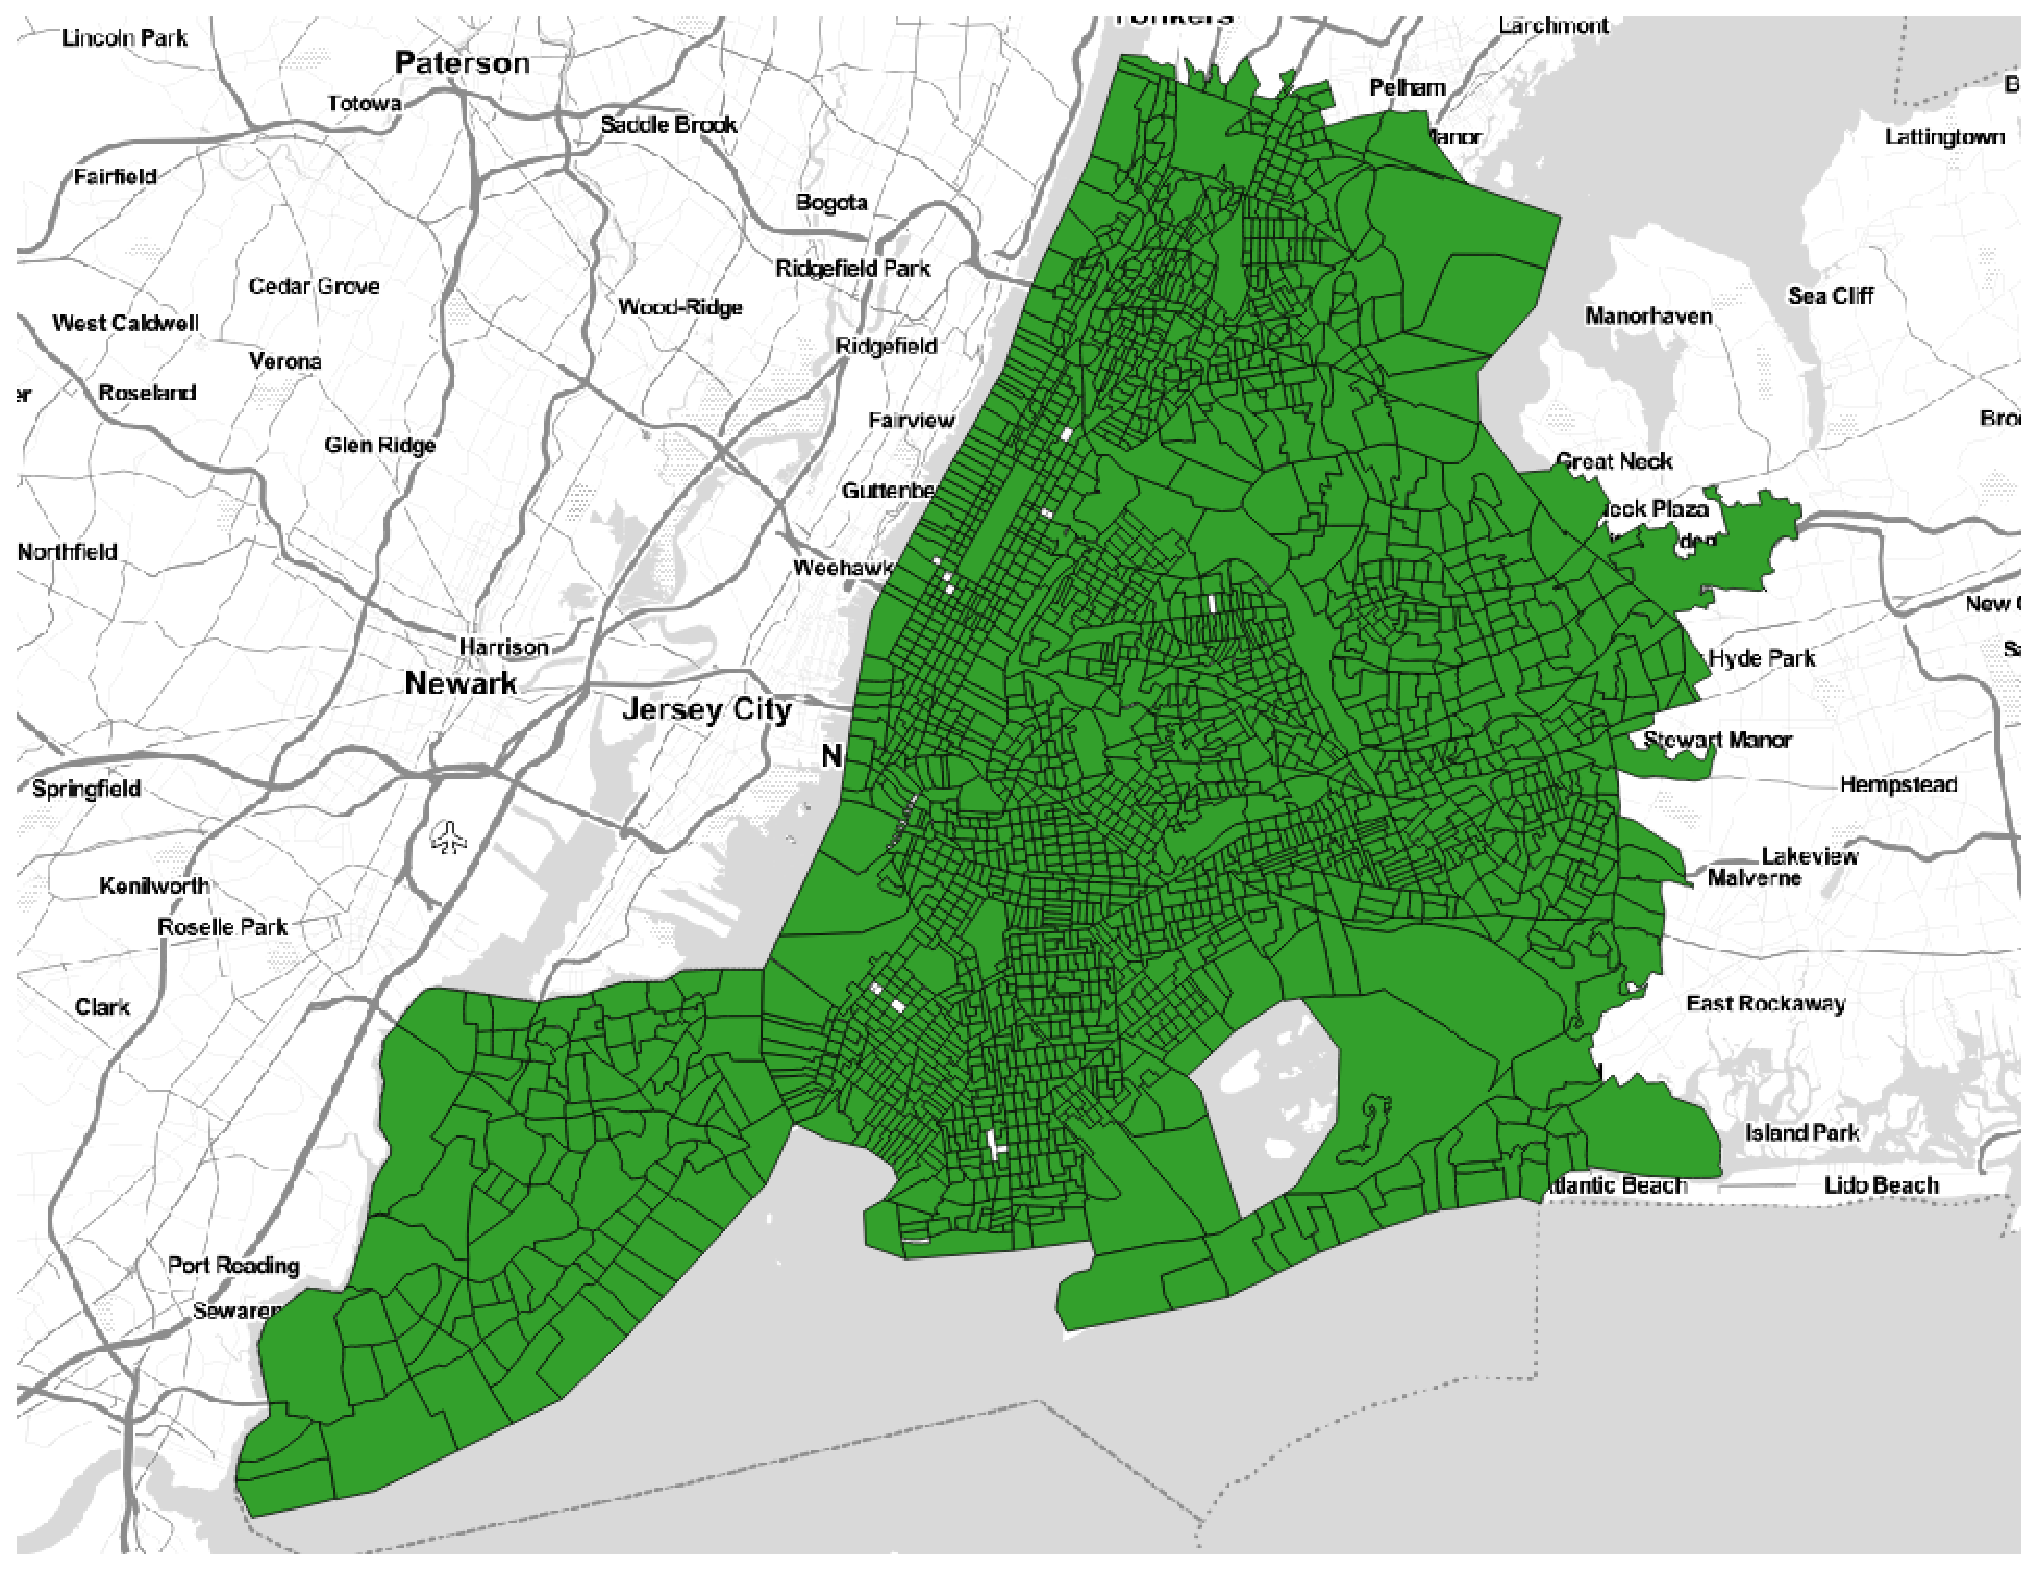
\includegraphics[width=\textwidth]{images/taxizone.eps}
		\caption{2,250 taxi analysis zone in New York City}
		\label{fig:taxizone}
	\end{subfigure}
	\hfill %add desired spacing between images, e. g. ~, \quad, \qquad, \hfill etc. 	%(or a blank line to force the subfigure onto a new line)
	\begin{subfigure}[b]{0.49\textwidth}
		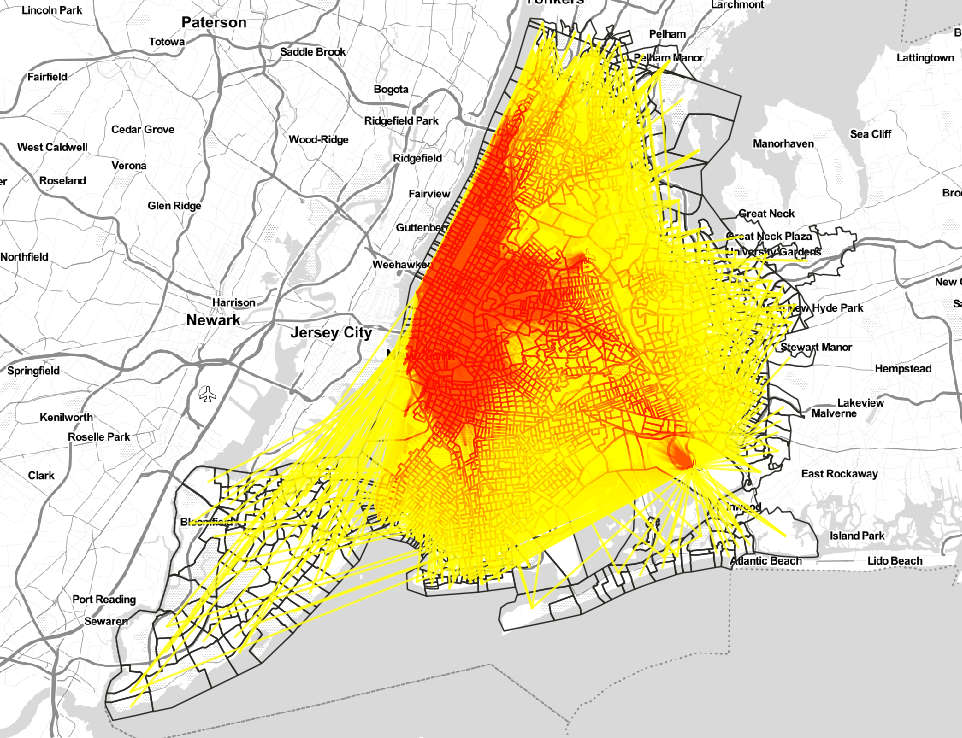
\includegraphics[width=\textwidth]{images/July1st_pic2.png}
		\caption{OD flows on July 01 2014}
		\label{fig:ODflows}
	\end{subfigure}
	\caption{Experimental data: New York City Taxi data}\label{fig:taxi_data}	
\end{figure}

As a case study, this study used OD trips for the comparison between weekdays and weekends in June. The weekdays data set includes taxi trajectories on June 3, 10, 17, and 24. There are 1,721,655 taxi trips. The weekends data set includes taxi trajectories on June 8, 15, 22, and 29.  Its taxi trips are 1,593,480. 

\subsection{Procedure}

The performance of the proposed method was compared with alternative methods. Trajectories anomalies detection, based on Mahalanobis distance \cite{pan13ACMSigspatial},  was used to compare the performance of outliers detection. The Mahalanobis distance considers the correlations of the data (e.g., two OD flows), which distinguishes it from Euclidean distance. According to \cite{pan13ACMSigspatial}, the anomaly detection threshold can be defined as below.

\begin{equation*}
d_M(OD_{t_1}, \mu_{[t_0,t_1)}) \geq 3\cdot \sqrt{\frac{1}{N}\sum_{t \in [t_0,t_1)} (OD_{t} - \mu_{[t_0,t_1)})^2} .
\end{equation*}

where $OD_{t_1}$ is the current OD flow, and $\mu_{[t_0,t_1)}$ is the median of all OD flows during $[t_0,t_1)$. In addition, we visualized the results in order to compare them and make the difference easier to understand. In terms of the difference of scale, we used standard statistics such as F-test to compare the variance of two groups.   

With regard to data cleaning process, this study used Hadoop with Pig. R was used to implement the code in Amazon Web Service  and Bridges supercomputer resources. Further, we used OD flows that have more than 10 trips. It is reasonable to remove the majority of low number of OD flows, which may distort the view of the data. 


%Data cleaning process

\subsection{Case study: weekdays vs weekends}
\subsubsection{Outlier Detection}
The bag plot presented OD flow outliers on weekdays and weekends separately in Figure \ref{fig:week_weekends_bag}. The outliers are detected by considering forward OD flows and reverse OD flow together. 


\begin{figure}
	\centering
	\begin{subfigure}[b]{0.49\textwidth}
		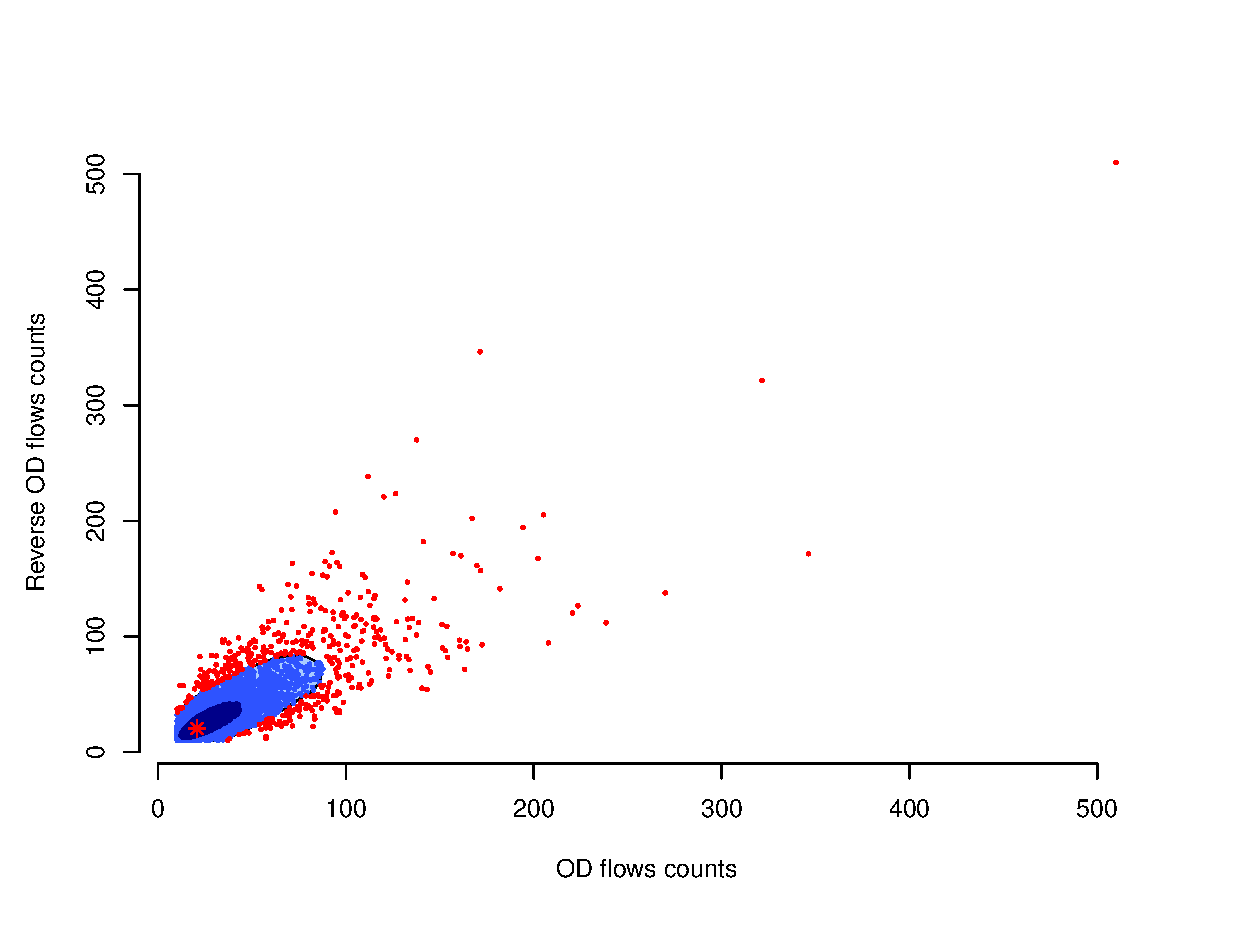
\includegraphics[width=\textwidth]{images/OD_weekdays.eps}
		\caption{Bag plot on weekdays}
		\label{fig:weekdays_bag}
	\end{subfigure}
	\hfill %add desired spacing between images, e. g. ~, \quad, \qquad, \hfill etc. 	%(or a blank line to force the subfigure onto a new line)
	\begin{subfigure}[b]{0.49\textwidth}
		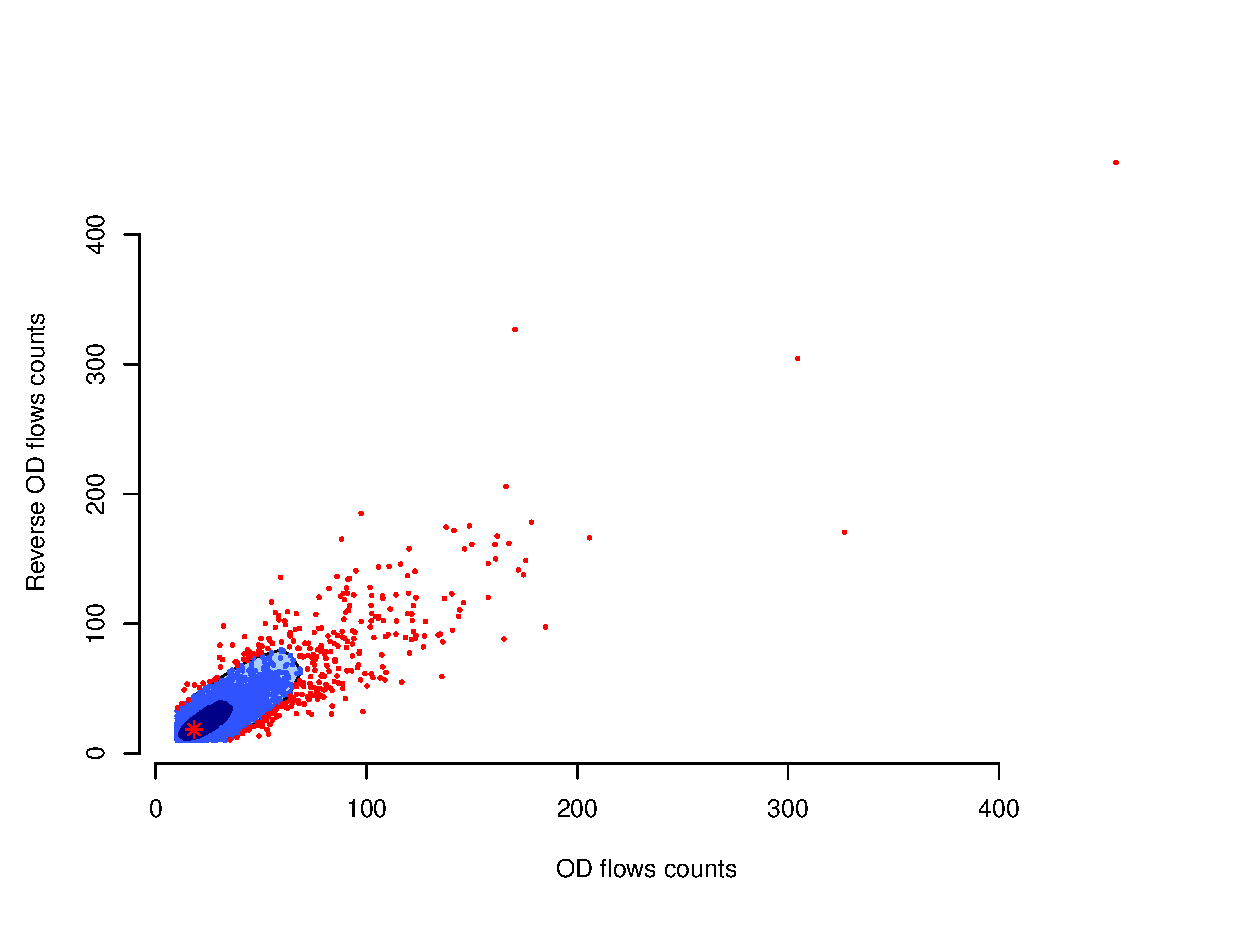
\includegraphics[width=\textwidth]{images/OD_weekends.eps}
		\caption{Bag plot on weekends}
		\label{fig:weekends_bag}
	\end{subfigure}
	\caption{Outliers detection of OD flows: X-axis indicates forward OD flows counts and Y-axis indicates reverse OD flows counts.}\label{fig:week_weekends_bag}	
\end{figure}

In order to find the difference between two data sets, we considered two forward OD flows together with the bag plot. Then we found the outliers of OD flows in Figure \ref{fig:weekdays_high}. In particular, the outliers with rectangle symbols indicates that these OD flows have high volume of taxi trips during weekdays and weekends. These outliers are superimposed on a map with red lines in Figure \ref{fig:weekdays_high_map}. The yellow lines presents OD flows except the high volume of OD flows on weekends. 

As this case very clearly demonstrated, the majority of OD flows occurred in broadly two places: within Manhattan, and between the center of Manhattan and two airports (i.e., J.F.K International airport and LaGuardia airport).  
 

\begin{figure}
	\centering
	\begin{subfigure}[b]{0.49\textwidth}
		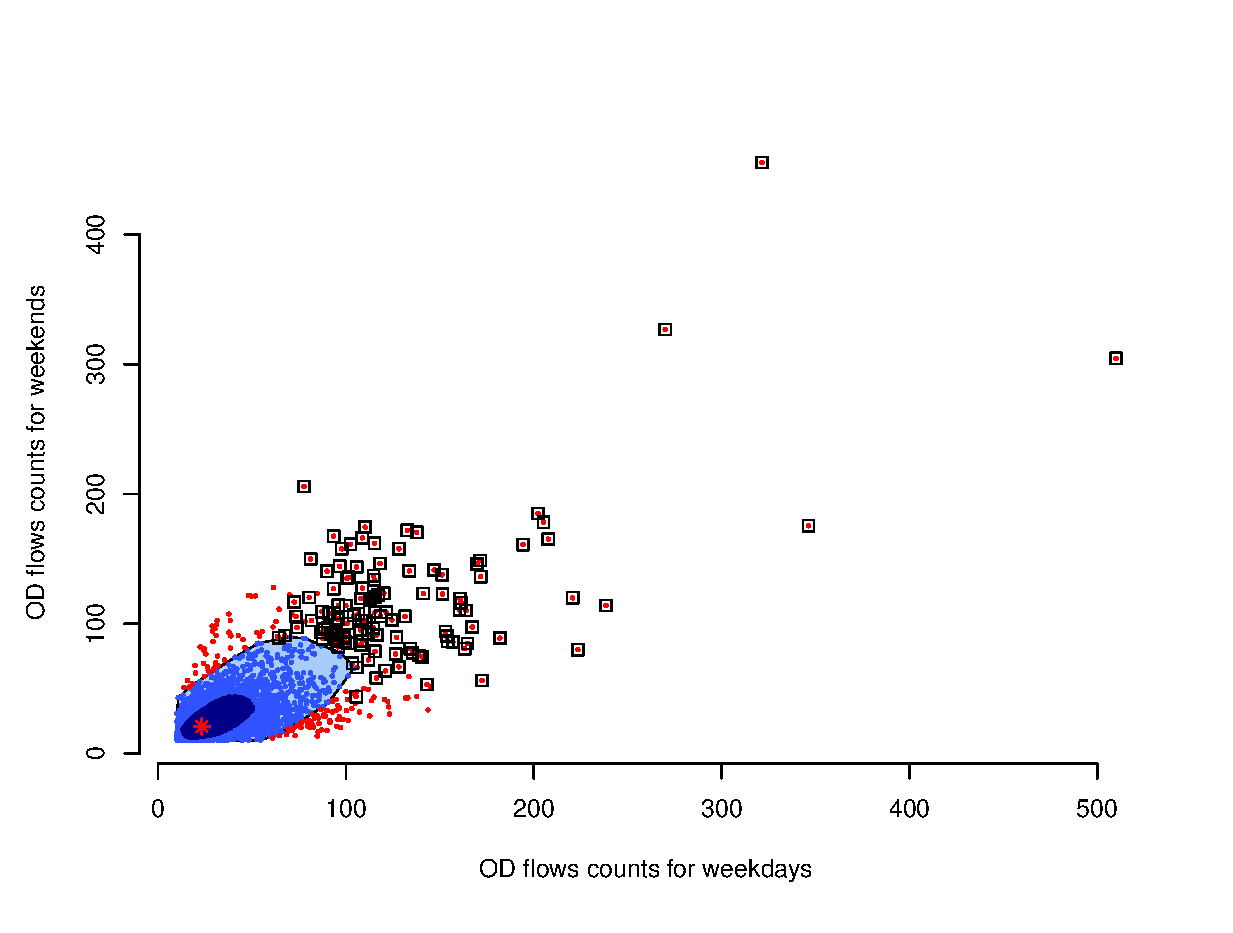
\includegraphics[width=\textwidth]{images/Outliers_high_weekdays_weekends.eps}
		\caption{High volume of OD flows}
		\label{fig:weekdays_high}
	\end{subfigure}
	\hfill %add desired spacing between images, e. g. ~, \quad, \qquad, \hfill etc. 	%(or a blank line to force the subfigure onto a new line)
	\begin{subfigure}[b]{0.49\textwidth}
		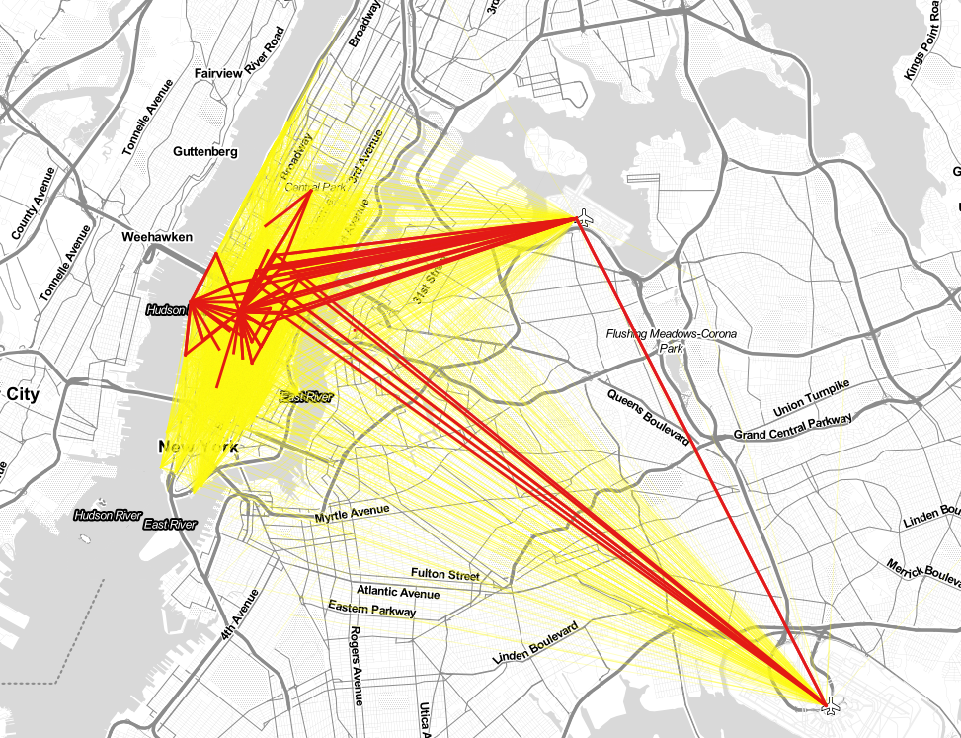
\includegraphics[width=\textwidth]{images/outliers2_high_weekdays_weekends.png}
		\caption{OD flow map for high volume of OD flows}
		\label{fig:weekdays_high_map}
	\end{subfigure}
	\caption{Outliers with high volume of trips on weekdays and weekends: Rectangles in Figure \ref{fig:weekdays_high} coincide with red lines in Figure \ref{fig:weekdays_high_map}. }\label{fig:weekdays_high_OD_map}	
\end{figure}

In addition, we investigated which OD flows are abnormal on weekends. They are typical OD flows on weekdays. These OD flows can have more taxi trips or less taxi trips compared with the OD flows on weekdays. Figure \ref{fig:weekdays_rare} presents these OD outliers with triangle symbols. These OD flows are represented on a map with red lines in Figure \ref{fig:weekdays_rare_map}.

\begin{figure}
	\centering
	\begin{subfigure}[b]{0.49\textwidth}
		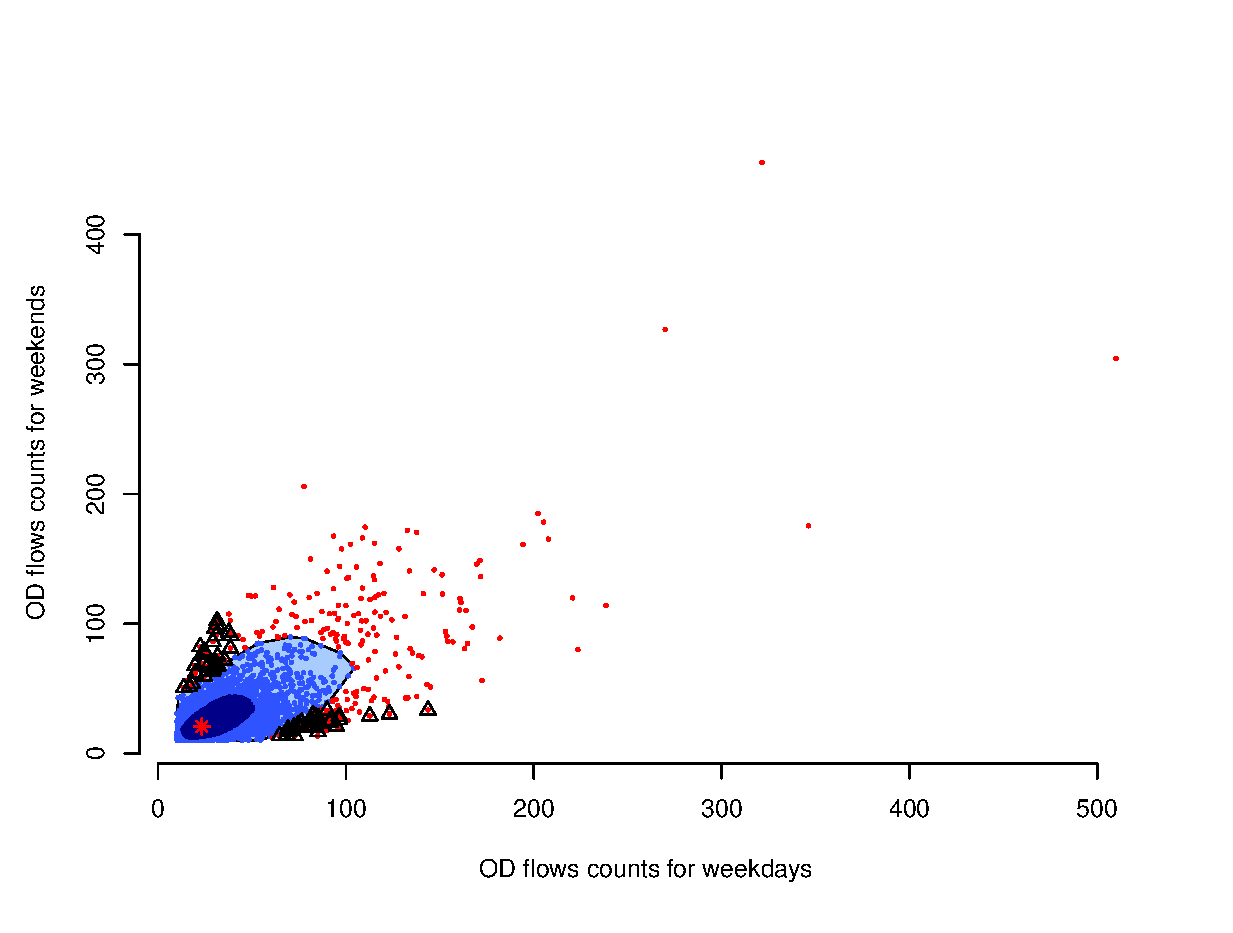
\includegraphics[width=\textwidth]{images/Outliers_rare_weekdays_weekends.eps}
		\caption{Relative OD outliers}
		\label{fig:weekdays_rare}
	\end{subfigure}
	\hfill %add desired spacing between images, e. g. ~, \quad, \qquad, \hfill etc. 	%(or a blank line to force the subfigure onto a new line)
	\begin{subfigure}[b]{0.49\textwidth}
		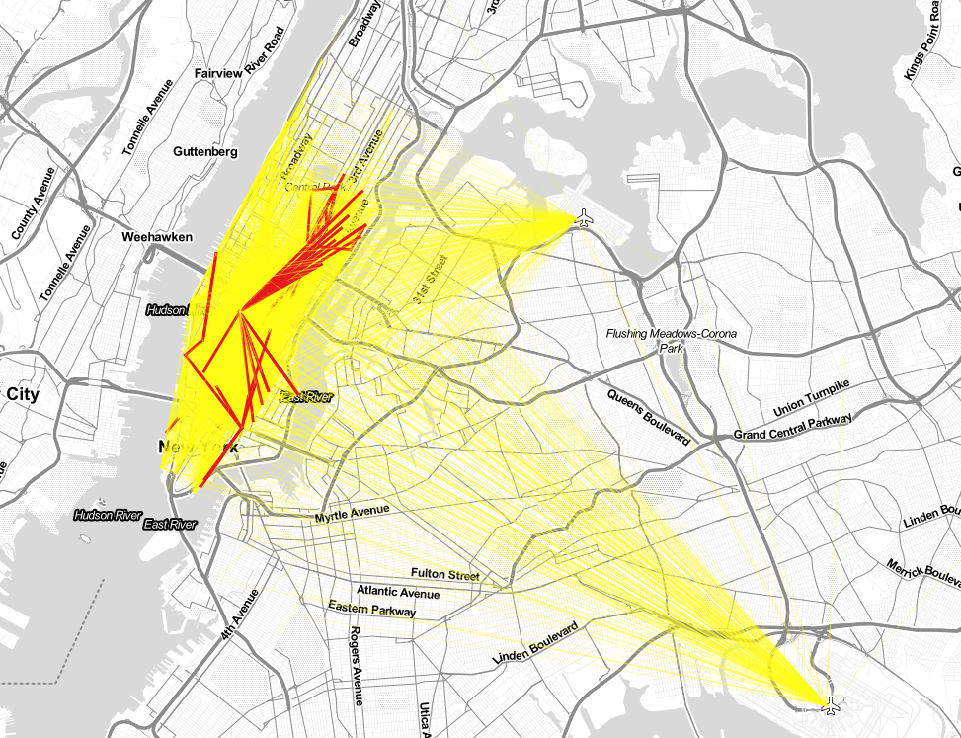
\includegraphics[width=\textwidth]{images/outliers_rare_weekdays_weekends.png}
		\caption{OD flow map for relative OD outliers}
		\label{fig:weekdays_rare_map}
	\end{subfigure}
	\caption{Relative OD outliers on weekdays and weekends: Triangles in Figure \ref{fig:weekdays_rare} coincide with red lines in Figure \ref{fig:weekdays_rare_map}. }\label{fig:weekdays_rare_OD_map}	
\end{figure}

Further, we detected OD outliers with Mahalanobis distance. The results are presented in Figure \ref{fig:week_ends_MD}. The number of OD outliers are very small compared with our approach. In particular, this method only considers forward OD flows with two data sets. It identified OD outliers with high volume of trips  because Mahalanobis distance takes into account the correlations between two OD flows. It is more likely to be outliers when two OD flows have high volume of trips. In fact, the OD outliers from Mahalanobis distance are the subset of them from our methods in Figure \ref{fig:weekdays_high_map}. 

\begin{figure}
	\centering
	\begin{subfigure}[b]{0.49\textwidth}
		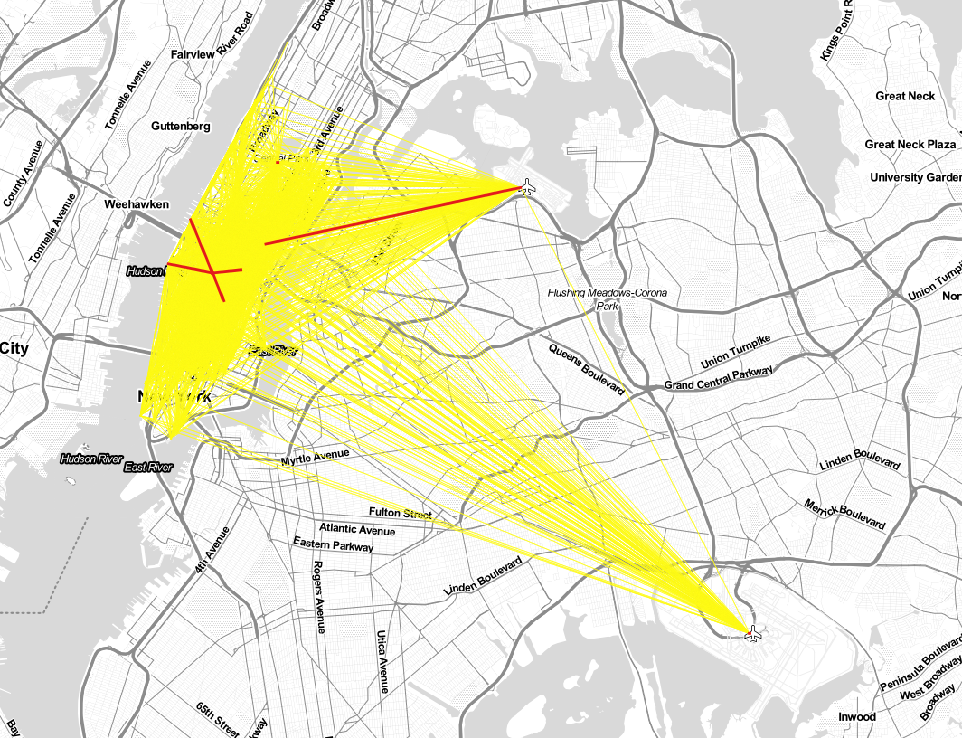
\includegraphics[width=\textwidth]{images/out_weekdays_weekends_md2_outlier.png}
	\end{subfigure}
	\caption{OD outliers on weekdays and weekends based on Mahalanobis distance. }\label{fig:week_ends_MD}	
\end{figure}

\subsubsection{Comparisons in scale}
We further investigated how two OD flows differ. Our approach is sensitive to the difference in scale. The hypothesis testing whether two central regions in Figure \ref{fig:OD_comparisons} are different by chance revealed that the confidence interval was -0.02769909 and 0.01573812, which includes zero. Thus, it failed to reject the null hypothesis. They were the same in terms of the spread.  

\begin{figure}
	\centering
	\begin{subfigure}[b]{0.7\textwidth}
		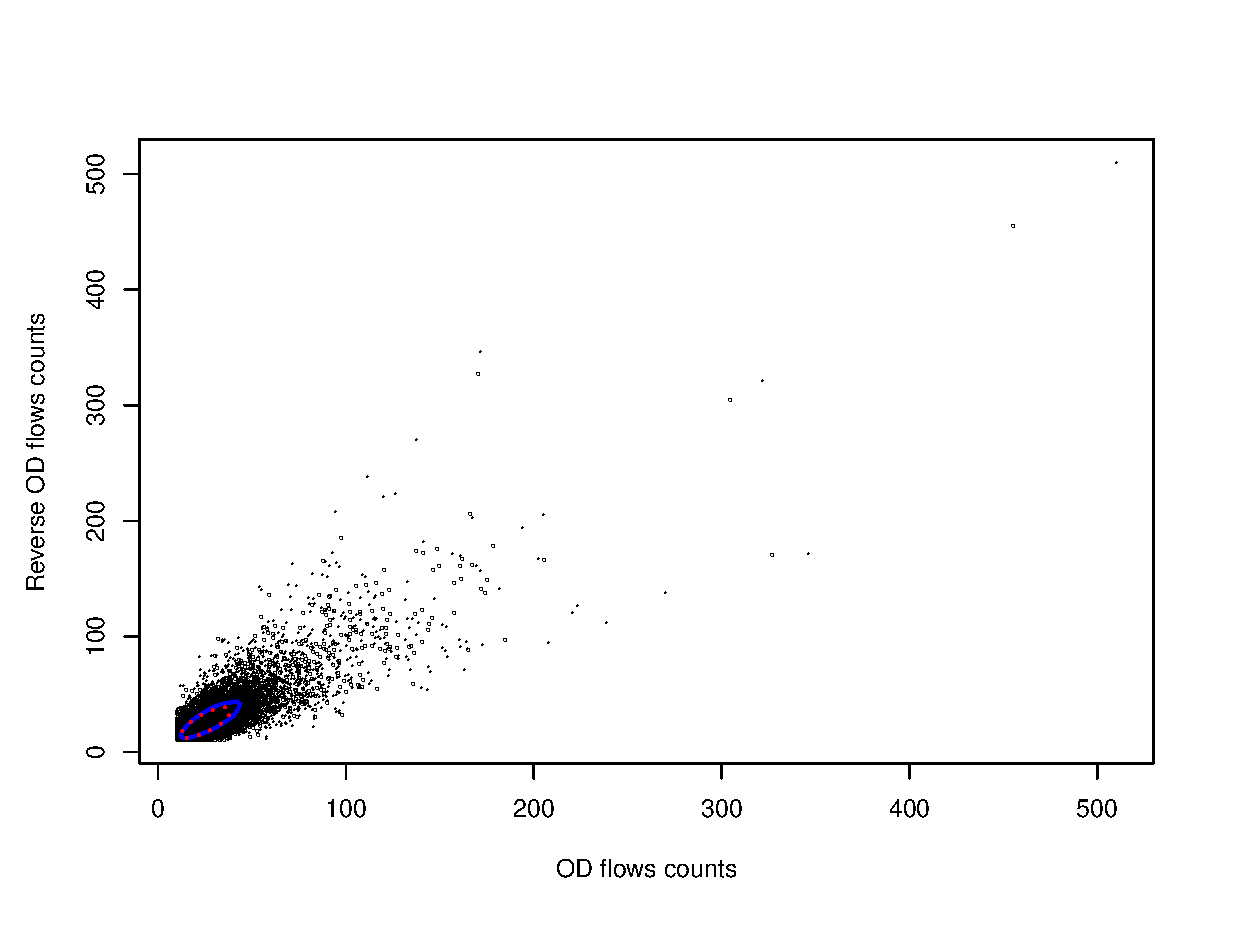
\includegraphics[width=\textwidth]{images/com_weekdays_weekends.eps}
	\end{subfigure}
	\caption{OD flows comparisons based on data depth: $\circ$ indicates the OD flows on weekdays and * indicates the OD flows on weekends; blue line presents the central region of the OD flows for the weekdays and red dotted line presents the central region of the OD flows on weekends. }\label{fig:OD_comparisons}	
\end{figure}

Interestingly, the standard statistic such as  F-test was significant, $F(9530,7637) =1.1786$, $p \leq 0.05$. The variances of two groups were significantly different. This is the opposite result compared with our approach. 


\subsection{Scalability}

\begin{figure}
	\centering
	\begin{subfigure}[b]{0.7\textwidth}
		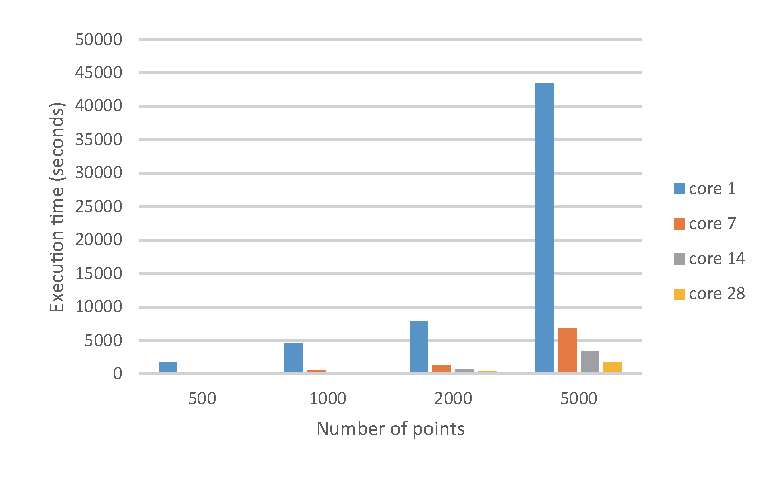
\includegraphics[width=\textwidth]{images/scalability.eps}
	\end{subfigure}
	\caption{Measure of time reduction. }\label{fig:scalability}	
\end{figure}

\section{Discussion}
\label{sec:discussion}
when the sample size is large, small differences in group differences can produce a F test is significant. 

This F-test is known to be extremely sensitive to non-normality,


\section{Conclusions and Future Work}
\label{sec:conclusions}
%the bag gives an idea of the shape of the majority of the data cloud.
%how to generalize: point-based approach.
%
%Tukey's depth makes no assumptions about the distribution from which observations are randomly sampled.  
%
%
%Outliers can be identified and treated in an interactive way.
%
%Multivariate depth statistics are particularly suited to analyze non-
%Gaussian or, more general, non-elliptical distributions in Rd . Without
%In inference, tests for
%goodness of fit and homogeneity regarding location, scale and symmetry are based
%on depth statistics




\subparagraph*{Acknowledgements.}



%%
%% Bibliography
%%

%% Please use bibtex, 

\bibliography{giscience2018}


\end{document}
